% !TEX root = ../dg.tex

\section{The Levi-Civita Connection}
\label{sec:levi-civita connection}

We need to define two notions, compatibility and symmetry, before we can give the main theorem of this section, which is the existence of the Levi-Civita connection.

\begin{definition}\label{def:compatible connection}
	Let $(M,g)$ be a Riemannian manifold with affine connection $\nabla$. The connection is called \emph{compatible} with $g$ if, for any smooth curve $\alpha$ and any pair of parallel vector fields $V$ and $W$ along $\alpha$, the function $t \mapsto g_{\alpha(t)}(V(t),W(t))$ is constant along $\alpha$.
\end{definition}

\begin{example}
	The Euclidean connection on $\R^n$ from \Cref{ex:euclidean connection} is compatible with the Euclidean metric since parallel vector fields are constant.
\end{example}

\begin{exercise}
	 Show that the restriction of the Eucliden connection to a submanifold $M^m \subset \R^n$ is compatible with the metric on $M$ induced by the Euclidean metric on $\R^n$.
\end{exercise}

\begin{exercise}\label{ex:compatibility and covariant differentiation}
	Show that an affine connection $\nabla$ is compatible with a Riemannian metric $g$ on $M$ if and only if, for any vector fields $V$ and $W$ along a smooth curve $\alpha \from I \to M$, we have
	\[
		\left.\frac{d}{dt}\right|_{t=t_0} g_{\alpha(t)}(V(t),W(t)) = g_{\alpha(t_0)} \left(\frac{DV}{dt},W\right) + g_{\alpha(t_0)} \left(V,\frac{DW}{dt}\right).
	\]
	In other words, for compatible connections we can use the usual product rule to differentiate the inner product.
\end{exercise}

\begin{corollary}\label{cor:compatibility equation}
	Let $(M,g)$ be a Riemannian manifold. An affine connection $\nabla$ on $M$ is compatible with $g$ if and only if 
	\begin{equation}\label{eq:compatibility}
		U(g(V,W)) = g(\nabla_UV,W) + g(V,\nabla_UW)
	\end{equation}
	at all points of $M$ and for all $U,V,W \in \mathfrak{X}(M)$.
\end{corollary}

\begin{proof}
	Suppose $\nabla$ is compatible with $g$. Let $p \in M$ and let $\alpha \from (-\epsilon,\epsilon) \to M$ be a smooth curve with $\alpha(0) = p$ and $\alpha'(0) = U(p)$. Then
	\begin{align*}
		U(g(V,W))(p) & = \left. \frac{d}{dt} \right|_{t=t_0} g_{\alpha(t)}(V,W) \\
		& = g_p\left(\frac{DV}{dt},W\right) + g_p\left(V,\frac{DW}{dt}\right) \\
		& = g_p(\nabla_{U(p)}V,W(p)) + g_p(V(p),\nabla_{U(p)}W),
	\end{align*}
	where the second line follows from \Cref{ex:compatibility and covariant differentiation} and the third from \Cref{prop:covariant derivative}\ref{it:cov der3}. Since $p$ was chosen arbitrarily, \eqref{eq:compatibility} follows.
	
	On the other hand, if $\nabla$ satisfies \eqref{eq:compatibility} and $V,W$ are parallel along $\alpha \from I \to M$, then \Cref{ex:compatibility and covariant differentiation} implies that
	\[
		\frac{d}{dt} g_{\alpha(t)}(V(t),W(t)) = g_{\alpha(t)} \left(\frac{DV}{dt},W\right) + g_{\alpha(t)} \left(V,\frac{DW}{dt}\right) = 0
	\]
	since $\frac{DV}{dt} \equiv 0$ and $\frac{DW}{dt} \equiv 0$.
\end{proof}

\begin{definition}\label{def:symmetric connection}
	A connection $\nabla$ on $M$ is called \emph{symmetric} or \emph{torsion-free} if 
	\[
		\nabla_V W - \nabla_W V = [V,W]
	\]
	for all $V,W \in \mathfrak{X}(M)$.
\end{definition}

\begin{example}
	Consider the Euclidean connection on $\R^n$ again (as defined in \Cref{ex:euclidean connection}). We use the standard coordinates on $\R^n$, and assume $V = \sum_i v_i \frac{\partial}{\partial x_i}$ and $W = \sum_j w_j \frac{\partial}{\partial x_j}$. Then
	\begin{align*}
		\nabla_VW & = \sum_{i,j} v_i \frac{\partial w_j}{\partial x_i} \frac{\partial}{\partial x_j} \\
		\nabla_WV & = \sum_{i,j} w_j \frac{\partial v_i}{\partial x_j} \frac{\partial}{\partial x_i},
	\end{align*}
	so we can match indices and conclude that
	\[
		\nabla_VW - \nabla_WV = \sum_{i,j} \left(v_i \frac{\partial w_j}{\partial x_i} - w_i \frac{\partial v_j}{\partial x_i}\right) \frac{\partial}{\partial x_j}.
	\]
	On the other hand, we saw way back in \eqref{eq:Lie bracket in local coords} that this is the local coordinate expression for $[V,W]$, so we see that the Euclidean connection is symmetric.
\end{example}

\begin{example}
	If we work in a local coordinate chart on a manifold $M$ and write $X_i = \frac{\partial}{\partial x_i}$, then $\nabla$ being symmetric implies
	\[
		\nabla_{X_i} X_j - \nabla_{X_j}X_i = [X_i,X_j] = 0;
	\]
	that is,
	\[
		\nabla_{X_i}X_j = \nabla_{X_j}X_i.
	\]
	In fact, it's not hard to show that $\nabla$ is symmetric if and only if the above equation holds; this explains the terminology \emph{symmetric}.
	
	Since the Christoffel symbols are defined by
	\[
		\nabla_{X_i}X_j = \sum_k \Gamma_{ij}^k X_k,
	\]
	the connection $\nabla$ is symmetric if and only if
	\[
		\Gamma_{ij}^k = \Gamma_{ji}^k
	\]
	for all $i,j,k$. In turn, we know from \Cref{ex:christoffel determines connection} that any choice of the Christoffel symbols $\Gamma_{ij}^k$ determines a connection, so we can construct all symmetric connections by choosing $n \binom{n+1}{2} = \frac{n^2(n+1)}{2}$ functions $\Gamma_{ij}^k$ so that $\Gamma_{ij}^k = \Gamma_{ji}^k$ for all $i,j,k$.
\end{example}

We are now ready to state and prove the main result:

\begin{theorem}[{Levi-Civita~\cite{levi-civitaNozioneDiParallelismo1916}}]\label{thm:levi-civita}
	Let $(M,g)$ be a Riemannian manifold. There exists a unique affine connection $\nabla$ so that
	\begin{enumerate}
		\item $\nabla$ is symmetric and
		\item $\nabla$ is compatible with $g$.
	\end{enumerate}
\end{theorem}

This connection is usually called the \emph{Levi-Civita connection} or the \emph{Riemannian connection}.

\begin{proof}
	First we prove uniqueness. So suppose there were some such connection $\nabla$. Then, for any $U,V,W \in \mathfrak{X}(M)$, \Cref{cor:compatibility equation} implies
	\begin{align}
		U(g(V,W)) & = g(\nabla_U V,W) + g(V,\nabla_U W) \label{eq:conn1}\\
		V(g(W,U)) & = g(\nabla_VW,U) + g(W,\nabla_VU) \label{eq:conn2}\\
		W(g(U,V)) & = g(\nabla_WU,V) + g(U,\nabla_WV). \label{eq:conn3}
	\end{align}
	Since the connection is symmetric, we know that
	\[
		\nabla_UV - \nabla_VU = [U,V]
	\]
	and similarly for other terms, so subtracting \eqref{eq:conn3} from the sum of \eqref{eq:conn1} and \eqref{eq:conn2} yields
	\begin{align*}
		U(g(V,W)) + V(g(W,U)) - W(g(U,V)) & = g([U,W],V) + g([V,W],U) + g(\nabla_UV + \nabla_VU,W) \\
		& = g([U,W],V) + g([V,W],U) + g([U,V],W) + 2 g(\nabla_VU,W).
	\end{align*}
	In other words,
	\begin{equation}\label{eq:levi-civita formula}
		g(\nabla_VU,W) = \frac{1}{2}\left[U(g(V,W)) + V(g(W,U)) - W(g(U,V)) - g([U,W],V) - g([V,W],U) - g([U,V],W)\right],
	\end{equation}
	which shows that $\nabla$ is uniquely determined by $g$. Hence, if it exists, $\nabla$ must be unique.\footnote{An alternative argument works in coordinates and gives explicit equations for the $\Gamma_{ij}^k$ in terms of the components $g_{ij}$ for the metric. This is directly analogous to the standard formulas for the Christoffel symbols on surfaces.}
	
	To prove existence, we can simply define $\nabla$ by \Cref{eq:levi-civita formula}; it is straightforward to check that $\nabla$ defined in this way is a symmetric, compatible connection.
\end{proof}

\begin{example}\label{ex:hyperbolic plane connection}
	Let's work out the Levi-Civita connection for the Riemannian metric on $\Aff^+(\R)$ that we defined in \Cref{ex:affine hyperbolic metric}. Recall that we can identify $\Aff^+(\R)$ with the upper half-plane $H = \{(x,y) \in \R^2 : y > 0\}$ and that the metric $g$ can be represented by the matrix
	\begin{align*}
		g_{(x,y)} \leftrightarrow \begin{bmatrix} g_{11}(x,y) & g_{12}(x,y) \\ g_{12}(x,y) & g_{22}(x,y) \end{bmatrix} = \begin{bmatrix} \frac{1}{y^2} & 0 \\ 0 & \frac{1}{y^2} \end{bmatrix}.
	\end{align*}
	Let $X = \frac{\partial}{\partial x}$ and $Y = \frac{\partial}{\partial y}$. Since these are coordinate fields, we know $[X,Y] = 0$, and we always have $[X,X] = 0$ and $[Y,Y] = 0$ for any vector fields. So half of the terms in \eqref{eq:levi-civita formula} vanish. 
	
	The matrix for $g$ is telling us that
	\[
		g_{(x,y)}(X,X) = \frac{1}{y^2}, \quad g_{(x,y)}(X,Y) = 0, \quad g_{(x,y)}(Y,Y) = \frac{1}{y^2},
	\]
	and hence that, using \eqref{eq:levi-civita formula}
	\begin{align*}
		g_{(x,y)}(\nabla_X X,X) & = \frac{1}{2}\left[ X(g_{(x,y)}(X,X)) + X(g_{(x,y)}(X,X)) - X(g_{(x,y)}(X,X))\right] \\
		& = \frac{1}{2}X(g_{(x,y)}(X,X)) \\
		& = \frac{1}{2} \frac{\partial}{\partial x}\left(\frac{1}{y^2}\right) \\
		& = 0
	\end{align*}
	and
	\begin{align*}
		g_{(x,y)}(\nabla_X X,Y) & = \frac{1}{2}\left[ X(g_{(x,y)}(X,Y)) + X(g_{(x,y)}(Y,X)) - Y(g_{(x,y)}(X,X))\right] \\
		& = \frac{1}{2}\left[X(0) + X(0) - Y\left(\frac{1}{y^2}\right)\right] \\
		& = -\frac{1}{2} \frac{\partial}{\partial y}\left(\frac{1}{y^2}\right) \\
		& = \frac{1}{y^3}.
	\end{align*}
	Therefore, for any $a$ and $b$,
	\begin{equation}\label{eq:affconn1}
		g_{(x,y)}(\nabla_X X,aX+bY) = \frac{b}{y^3}.
	\end{equation}
	On the other hand, $\nabla_X X = cX+dY$ for some $c$ and $d$, and we know that
	\begin{equation}\label{eq:affconn2}
		g_{(x,y)}(cX+dY,aX+bY) = \frac{ac}{y^3} + \frac{bd}{y^3}.
	\end{equation}
	Equating \eqref{eq:affconn1} and \eqref{eq:affconn2}, we see that $\nabla_XX = \frac{1}{y}Y$.
	
	If we play the same game with $\nabla_YY$ and with $\nabla_XY = \nabla_YX$ (using the symmetry of $\nabla$ and the fact that $[X,Y] = 0$), we conclude that
	\begin{equation}\label{eq:hyperbolic plane Christoffel}
		\nabla_XX = \frac{1}{y}Y , \quad \nabla_XY = \nabla_YX = -\frac{1}{y}X, \quad \nabla_YY = -\frac{1}{y}Y.
	\end{equation}
	
	Now, let's think about parallel transporting a vector along the curve $\alpha(t) = (t,1)$. Notice that $\alpha'(t) = X$ for all $t$, so by \Cref{prop:covariant derivative}\ref{it:cov der3}, we have that the covariant derivative along $\alpha$ is given by
	\[
		\frac{DW}{dt} = \nabla_{\alpha'(t)} W = \nabla_X W
	\]
	for any tangent vector $W$. So if we think of a vector field $W(t) = a(t)X + b(t)Y \in T_{\alpha(t)}H = T_{(t,1)}H$, then the parallel transport equation becomes
	\begin{multline*}
		0 = \frac{DW}{dt} = \nabla_X (a(t)X + b(t)Y) = a'(t) X + a(t) \nabla_X X + b'(t)Y + b(t) \nabla_X Y \\
		= a'(t) X +a(t)Y + b'(t) Y - b(t)X = (a'(t)-b(t))X + (b'(t)+a(t))Y
	\end{multline*}
	since $y=1$ along the whole curve and hence $\frac{1}{y} = 1$. Of course, the coefficients have to be 0, so we get the homogeneous system of ODEs
	\begin{align*}
		a'(t)-b(t) & = 0 \\
		b'(t)+a(t) & = 0.
	\end{align*}
	Solutions are of the form
	\begin{align*}
		a(t) & = C_1 \cos t + C_2 \sin t \\
		b(t) & = -C_1 \sin t + C_2 \cos t.
	\end{align*}
	\Cref{fig:hpt} shows the parallel transports of $X \in T_{(0,1)}H$ and $Y \in T_{(0,1)}H$ along this curve.
	\begin{figure}[htbp]
		\centering
			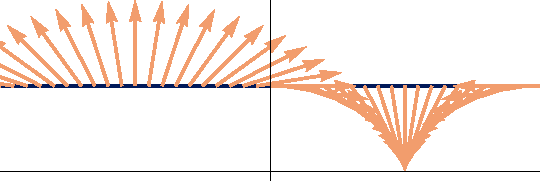
\includegraphics[height=.8in]{hpt2}
			\qquad 
			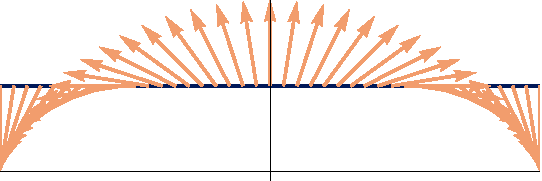
\includegraphics[height=.8in]{hpt1}
		\caption{The parallel transports of $X \in T_{(0,1)}H$ (left) and $Y \in T_{(0,1)}H$ (right) along the curve $\alpha(t) = (t,1)$.}
		\alttext{Two diagrams, each showing a horizontal line and a sequence of arrows indicating a vector field along the line. In both diagrams the vectors are rotating clockwise.}
		\label{fig:hpt}
	\end{figure}
	
	Recall that a parallel vector field is always pointing in the same direction from the perspective of someone inside the manifold, so the way to interpret this is that a person traversing the curve $\alpha(t)$ is constantly turning to the left to stay on $\alpha$.
	
	On the other hand, if $\beta(t) = (0,t)$, then $\beta'(t) = Y$ for all $t$, and the parallel transport equation is
	\begin{multline*}
		0 = \frac{DW}{dt} = \nabla_Y (a(t)X + b(t)Y) = a'(t) X + a(t) \nabla_Y X + b'(t)Y + b(t) \nabla_Y Y \\
		= a'(t) X -\frac{a(t)}{t}X + b'(t) Y - \frac{b(t)}{t}Y = \left(a'(t)-\frac{a(t)}{t})\right)X \left(b'(t)-\frac{b(t)}{t}\right)Y
	\end{multline*}
	since $y = t$ along the curve, and hence $\frac{1}{y} = \frac{1}{t}$. So the system of ODEs is
	\begin{align*}
		a'(t)-\frac{a(t)}{t} & = 0 \\
		b'(t)-\frac{b(t)}{t} & = 0.
	\end{align*}
	Solutions are of the form
	\begin{align*}
		a(t) & = C_1t \\
		b(t) & = C_2t.
	\end{align*}
	\Cref{fig:hpt2} shows the parallel transports of $X \in T_{(0,1)}H$ and $Y \in T_{(0,1)}H$ along this curve.
	\begin{figure}[htbp]
		\centering
			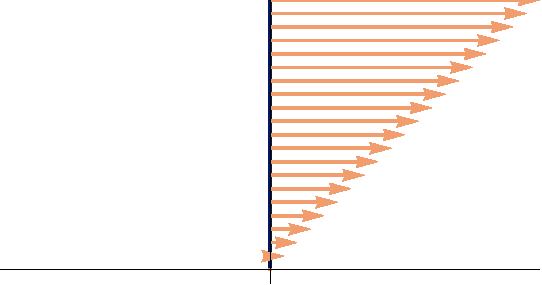
\includegraphics[height=1in]{hpt3}
			\qquad 
			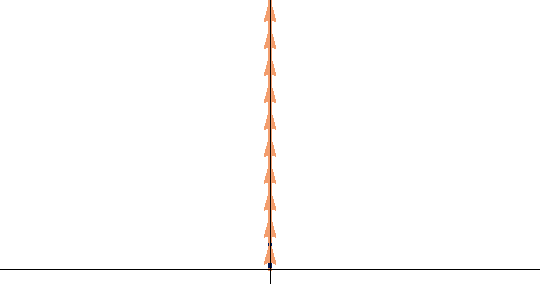
\includegraphics[height=1in]{hpt4}
		\caption{The parallel transports of $X \in T_{(0,1)}H$ (left) and $Y \in T_{(0,1)}H$ (right) along the curve $\beta(t) = (0,t)$.}
		\alttext{Two diagrams, each showing a vertical line and a sequence of arrows indicating a vector field along the line. In the first diagram the vectors are always pointing right, and in the second they always pointing up. In both cases, the vectors are getting longer as they go up.}
		\label{fig:hpt2}
	\end{figure}
	
	Notice that the parallel transport of a tangent vector to $\beta$ stays tangent to $\beta$; this is an indication that (up to reparametrization) $\beta$ is a geodesic.
\end{example}